\fancyhead[LO, RE] {Sviluppo}
\lstset{
showstringspaces=false
}
\lstdefinestyle{base}{
language=C,
  emptylines=1,
  breaklines=true,
  basicstyle=\ttfamily\color{black},
  moredelim=**[is][\color{blue}]{^}{^},
moredelim=**[is][\color{olive}]{<}{<},
moredelim=**[is][\color{magenta}]{£}{£},
moredelim=**[is][\color{red}]{!}{!},
moredelim=**[is][\color{violet}]{?}{?},
}
\section{Sviluppo}
\subsection{Sviluppo programma di export}
\subsubsection{Architettura della solizione}
La versione iniziale del programma di export è stata sviluppata nel 2007 da uno dei programmatori attualmente presenti in azienda e si basa sulla creazione di file di testo che vengono inviati al fornitore, perché si occupi di caricare i database degli showroom della campagna vendite.\\
Dato che la decisione per l'upgrade è stata quella di utilizzare dei DbLink, sotto consiglio del tutor aziendale il primo passo è stato creare una copia esatta delle tabelle dei database di destinazione, all'interno del database di sviluppo, sul quale è stato sviluppato il prototipo. Il motivo della copia è che al momento della scrittura remota tramite dblink sarebbe stato molto più semplice fare un riversamento del contenuto di una tabella all'interno di un'altra, ed in puù in questo modo si ha una versione di backup locale dei dati, in modo che se ci dovessero essere errori nel trasferimento, utilizzando i vari sistemi di tracciamento adottati, che vedremo in seguito nello specifico, si può correggere facilmente ogni problematica. Inoltre in un sistema Eterogeneo (ovvero collegamento fra database server di tipo diverso, Oracle to Sql Server) non si possono eseguire manipolazioni dei dati all'interno delle query di inserimento, come ad esempio conversioni o formattazioni, che vengono quindi anticipate alla fase di caricamento nella parte locale.\\
Una volta create tutte le tabelle locali, il passo successivo è stato prendere spunto dalle query del programma esistente ed ottenere tutti i dati necessari a ricreare le nuove query, con alcune modifiche proposte dai service manager, per popolarle. L'esecuzione del programma prevede anche degli input che talvolta possono essere facoltativi, ma la loro presenza va considerata all'interno delle query e ciò comporta l'utilizzo dei \textbf{refcursor} per permettere una parametrizzazione della query.\\
Durante il popolamento della tabella locale, viene valorizzato il campo di log 'Data\_modifica' che verrà in seguito utilizzato per capire quali dati riversare nel database remoto, confrontandola con la data impostata all'inizio di esecuzione del programma.
\subsubsection{Codice}
Di seguito vediamo la porzione di codice che mostra il percorso di estrazione dati, popolamento della tabella locale ed infine popolamento della tabella remota relativa ai Modelli.\\
Il primo passo è la definizione di una stringa di testo che in Run-Time sarà query eseguibile, contente l'interrogazione esatta necessara:
\begin{lstlisting}[frame=single, style=base]
?v_query? := 
'Select Distinct 
    substr(m.ogg_cod,6,5)   cd_modello,'     || chr(10) ||
'   substr(m.ogg_cod,11,2)   cd_varia,'      || chr(10) ||
'   ''C''  TipoAna,'                         || chr(10) ||
'   substr(m.ogg_cod,1,5)  cd_Ana,'          || chr(10) ||
'    m.ogg_des Descrizion,'                  || chr(10) ||
'   ''STD''  cd_defmod,'                     || chr(10) ||
'   m.ogg_stg_anno||
    Substr(m.ogg_stg_cod,1,1) cd_stagion,'   || chr(10) ||
'   Substr(ms.ogg_soc_lin_cod,1,3) cd_lin ,' || chr(10) ||
'   tg.tgl_ogg_grt_cod cd_Taglia,' 	     || chr(10) ||
'   null cd_Flash,' 	                     || chr(10) ||
'   null cd_Colle,' 		             || chr(10) ||
'   0    qtaconf,' 		             || chr(10) ||
'   m.ogg_cod   cd_modello_ex,' 	     || chr(10) ||
'   nvl(m.ogg_f_annu,''0'') mod_flannu'      || chr(10) ||
'  From s3t_ogg_soc ms,
            s3t_tgl_ogg tg, 
           s3t_ogg m' || chr(10) ||
' Where ms.ogg_soc_soc_cod(+)=
   s3ksysutils.SocPubPriv('''||^s3ksysglobal^.Soc_Ute||''',
                               ''OGG_SOC'')' || chr(10) ||
'And ms.ogg_soc_ogg_soc_cod(+)=
            m.ogg_soc_cod' || chr(10) ||
'And ms.ogg_soc_ogg_id(+)=
            m.ogg_id' || chr(10) ||
'And tg.tgl_ogg_ogg_soc_cod(+)=
            m.ogg_soc_cod' || chr(10) ||
'And tg.tgl_ogg_ogg_id(+)=
            m.ogg_id' || chr(10) ||
'And m.ogg_tipo=''1''' || chr(10) ||
'AND (to_char(m.ogg_data_mod,''YYYY/MM/DD HH24:MI:SS'') >
'''||to_char(?LastExcutionData?,'YYYY/MM/DD HH24:MI:SS')
||''''||
        chr(10) ||
'        OR' || chr(10) ||
'to_char(ms.ogg_soc_data_mod,''YYYY/MM/DD HH24:MI:SS'') >
'''||to_char(?LastExcutionData?,'YYYY/MM/DD HH24:MI:SS')

'        OR' || chr(10) ||
'to_char(tg.tgl_ogg_data_mod,''YYYY/MM/DD HH24:MI:SS'') >
'''||to_char(?LastExcutionData?,'YYYY/MM/DD HH24:MI:SS')
||''')'||
        chr(10) ||
'And m.ogg_stg_anno||''/''||m.ogg_stg_cod =
       '''||?P_STG_ATT?||'''';

IF v_mrc_lis IS NOT NULL THEN
  ?v_query? := ?v_query? ||'
             And Substr(ms.ogg_soc_lin_cod,1,2)
                 in ('''||?v_mrc_lis?||''')  ORDER BY 1';
END IF;
IF v_lnv IS NOT NULL THEN
  ?v_query? := ?v_query? ||
             ' And ms.ogg_soc_lin_cod 
                  in ('''||?v_lnv?||''')';  
END IF;
\end{lstlisting}
La sintassi di PL/SQL prevede che la concatenazione fra stringhe di testo (delimitate da apici) avvenga tramite il 'pipe' due volte in successione, inoltre l'inserimento di una variabile all'interno della stringa va gestito con cautela, in quanto va fatta una distinzione sul tipo della variabile inserita: \\
\begin{itemize}
\item se è di tipo alfanumerico vanno utilizzati 3 apici in chiusura della stringa, seguiti dalla variabile ed a sua volta seguita da altri 3 apici, ogni parte concatenata con l'altra; questo perché ci deve essere una forma di escape tra gli apici che distinguono il testo della query in stato di stringa ed il contenuto della variabile, che in Run-Time, quando viene effettivamente eseguita la query, diventa un valore alfanumerico senza significato per un compilatore, non utilizzabile in un confronto o una selezione.\\
\item se è di tpo intero basta una concatenazione senza apici aggiuntivi
\end{itemize}

La fase successiva all'estrazione dei dati è quella di caricarli nella tabella locale dei Modelli.
\begin{lstlisting}[frame=single,style=base]
^open^ ?Cur_mod? ^for^ ?v_query?;
  ^LOOP^
    ^fetch^ ?Cur_mod? ^into^ ?cd_modello_mod?,
                       ?cd_varia_mod?,
                       ?TipoAna_mod?,
                       ?cd_Ana_mod?,
                       ?Descrizion_mod?,
                       ?cd_defmod_mod?,
                       ?cd_stagion_mod?,
                       ?cd_lin_mod?,
                       ?cd_taglia_mod?,
                       ?cd_flash_mod?,
                       ?cd_Colle_mod?,
                       ?qtaconf_mod?,
                       ?cd_modello_ex_mod?,
                       ?mod_flannu_mod?;
    ^exit when^ ?Cur_mod?%^notfound^;
    ^BEGIN^
      <INSERT INTO< PINDT_MOD_CRM(cd_modello,
                                cd_varia,
                                tipoana,
                                cd_ana,
                                descrizion,
                                cd_defmod,
                                cd_stagion,
                                cd_linea,
                                cd_taglia,
                                cd_flash,
                                datains,
                                dataupd,
                                annullato,
                                qtaconf,
                                cd_modello_ex,
                                societa
                                )
                         <VALUES<(?Cd_Modello_mod?,
                                ?Cd_Varia_mod?,
                                ?TipoAna_mod?,
                                ?Cd_Ana_mod?,
                                ?Descrizion_mod?,
                                ?cd_defmod_mod?,
                                ?Cd_Stagion_mod?,
                                ?Cd_Lin_mod?,
                                ?Cd_Taglia_mod?,
                                ?Cd_Flash_mod?,
                                ?LastExcutionData?,
                                ?v_sysd?,
                                ?Mod_Flannu_mod?,
                                ?Qtaconf_mod?,
                                ?Cd_Modello_Ex_mod?,
                                ^s3ksysglobal^.Soc_Ute
                                );
    ^exception^
      ^when^ dup_val_on_index ^then^
        ^BEGIN^
          <Update< Pindt_Mod_Crm t 
             <Set< t.Descrizion     = ?Descrizion_mod?,
                 t.cd_defmod      = ?Cd_Defmod_mod?,
                 t.cd_stagion     = ?Cd_Stagion_mod?,
                 t.cd_linea       = ?Cd_Lin_mod?,
                 t.cd_flash       = ?Cd_Flash_mod?,
                 t.dataupd        = ?v_sysd?,
                 t.annullato      = ?Mod_Flannu_mod?,
                 t.qtaconf        = ?Qtaconf_mod?,
                 t.cd_modello_ex  = ?Cd_Modello_Ex_mod?
           <Where< t.cd_modello   = ?Cd_Modello_mod?
             <and< t.cd_varia     = ?Cd_Varia_mod?
             <and< t.tipoana      = ?Tipoana_mod?
             <and< t.cd_ana       = ?Cd_Ana_mod?
             <and< t.societa      = ^s3ksysgloba^l.Soc_Ute;
        ^exception when others then^
            v_error := !sqlerrm!;
            ^s3ksysmess.Batch_Messaggi^(£60070£,^sysdate^,
	'MODELLI:'||^nvl^(?Cd_Modello_mod?,'codice null'));
        ^END^;
      ^when others then^
        v_error := !sqlerrm!;
        ^s3ksysmess.Batch_Messaggi^(£60070£,^sysdate^,
	'MODELLI:'||^nvl^(?Cd_Modello_mod?,'codice null'));
    ^END^;
    ^commit^;
  ^END LOOP^;
  ^close^ ?Cur_mod?;
\end{lstlisting}

In questo blocco di codice possiamo vedere un'applicazione dei refcursor, il cui contenuto viene iterato per ogni record estratto dalla query definita sopra, ed ogni riga viene utilizzata come testata per un secondo cursore interno, il quale estrae tutti i colori disponibili per quel modello-parte.\\
Si può inoltre vedere una gestione degli errori, permessa dalla struttura \textbf{BEGIN/exception/END} di PLSQL, in cui un errore di tipo 'chiave logica duplicata' viene gestito con un ulteriore blocco in cui viene aggiornato il valore del record per la chiave estratta. Eventuali errori generici vengono gestiti con un sistema di messaggistica sottoforma di Log, messo a disposizione da Stealth.\\
All'inizio della funzione che contiene i due blocchi di codice precedenti, viene assegnato il valore della data attuale alla variabile v\_sysd grazie alla keyword \textbf{sysdate}, e quest'ultima sarà il filtro per decidere quali valori della tabella locale verranno trasferiti nel database remoto, come si vede nel seguente blocco di codice finale:
\begin{lstlisting}[frame=single, style=base]
^BEGIN^
  ^FOR^ ?CUR_MOD? ^IN^ (
             ^SELECT^ * 
               ^FROM^ PINDT_MOD_CRM t 
              ^WHERE^ t.dataupd = ?v_sysd? 
                ^and^ t.societa = ^s3ksysglobal^.Soc_Ute
                ^AND^ t.cd_stagion = 
                    replace(?P_STG_ATT?,'/')) 
  ^LOOP^
    ^BEGIN^
      ?v_qtaconf? := ^to_number^(?Cur_mod?.Qtaconf);
      <INSERT INTO< modelli@crm_sydat_eur.industries.com(
                  "Cd_modello",
                  "Cd_Varia",
                  "TipoAna",
                  "Cd_Ana",
                  "Descrizion",
                  "Cd_Defmod",
                  "Cd_Stagion",
                  "Cd_linea",
                  "Cd_Taglia",
                  "Cd_Flash",
                  "Cd_Colle",
                  "QtaConf",
                  "DataUpd",
                  "DataIns",
                  "Annullato",
                  "cd_modello_ex"
                  )
           <VALUES<(?Cur_mod?.Cd_Modello,
                  ?Cur_mod?.Cd_Varia,
                  ?Cur_mod?.Tipoana,
                  ?Cur_mod?.Cd_Ana,
                  ?Cur_mod?.Descrizion,
                  ?Cur_mod?.Cd_Defmod,
                  ?Cur_mod?.Cd_Stagion,
                  ?Cur_mod?.Cd_Linea,
                  ?Cur_mod?.Cd_Taglia,
                  ?Cur_mod?.Cd_Flash,
                  ?Cur_mod?.Cd_Colle,
                  ?v_qtaconf?,
                  ?v_date?,
                  ?v_date?,
                  ?Cur_mod?.Annullato,
                  ?Cur_mod?.Cd_Modello_Ex                                                  
                  );
       ^commit^;
       ?v_modelli_ins? := ?v_modelli_ins? + 1;
    ^exception^
     ^when^ Dup_insert ^then^
       ^BEGIN^



        <UPDATE< modelli@crm_sydat_eur.industries.com 
           <SET< "Descrizion" = ?Cur_mod?.Descrizion,
               "Cd_Defmod" = ?Cur_mod?.Cd_Defmod,
               "Cd_Stagion" = ?Cur_mod?.Cd_Stagion,
               "Cd_linea" = ?Cur_mod?.Cd_Linea,
               "Cd_Taglia" = ?Cur_mod?.Cd_Taglia,
               "Cd_Flash" = ?Cur_mod?.Cd_Flash,
               "Cd_Colle" = ?Cur_mod?.Cd_Colle,
               "QtaConf" = ?Cur_mod?.Qtaconf,
               "DataUpd"       = ?v_date?,
               "Annullato"     = ?Cur_mod?.Annullato,
               "cd_modello_ex" = ?Cur_mod?.Cd_Modello_Ex
         <WHERE< "Cd_modello" = ?Cur_mod?.Cd_Modello
           <AND< "Cd_Varia" = ?Cur_mod?.Cd_Varia
           <AND< "TipoAna" = ?Cur_mod?.Tipoana
           <AND< "Cd_Ana" = ?Cur_mod?.Cd_Ana;
            ^commit^;
                                                  
           ?v_modelli_upd? := ?v_modelli_upd? + 1;
        ^exception when others then^
          ?v_error? := !sqlerrm!;
          ^s3ksysmess.Batch_Messaggi^(£60071£,^sysdate^,'Modelli'||!sqlerrm!);
          ?v_modelli_err? := ?v_modelli_err? + 1;
          ^rollback^;
        ^END^;
      ^when others then^
        ?v_error? := !sqlerrm!;
        s3ksysmess.Batch_Messaggi(£60071£ ,sysdate,'Modelli'||!sqlerrm!);
        ?v_modelli_err? := ?v_modelli_err? + 1;
        ^rollback^;
    ^END^;
  ^END LOOP^;
  ^exception when others then^
      ^s3ksysmess.Batch_Messaggi^(£1583£,^sysdate^,'Modelli: ',!sqlerrm!);
    ^END^;
\end{lstlisting}
In un sistema Eterogeneo, ovvero in cui i database collegati dal DbLink sono diversi, come in questo caso tra Oracle e Sql Server, il riferimento ai campi dati di una tabella remota vanno specificati utilizzando il doppio apice ad inizio e fine, ed il nome è \textit{case sensitive}.\\
I dati estratti dal cursore per essere riversati nella tabella remota sono filtrati per la data impostata precedentemente, in fase di caricamento della tabella locale.
Quanto emerso da elaborazioni su set ristretti di dati, i DbLink in un sistema eterogeneo sono piuttosto lenti, nel caso specifico vengono trasferiti circa 1200 record al secondo in inserimento, mentre circa la metà in fase di modifica data la presenza di condizioni di filtro (nella clausola WHERE) che necessariamente rallentano l'esecuzione. Inoltre la decisione di eseguire una \textbf{commit} ad ogni record, utile per avere dei dati in fase di esecuzione in caso il programma sia molto lungo nella sua esecuzione, rallenta il processo, rispetto ad avere una singola commit alla fine dell'esecuzione, al costo ovviamente di non aver inserito nessuna riga in caso di un qualsiasi errore.\\
Nel complesso, l'autonomia dell'esecuzione, e soprattutto la decisione di schedulare il programma ogni notte per rendere marginale la questione della velocità di esecuzione, permettono di avere un vantaggio rispetto alla versione attuale del programma.
\subsection{Sviluppo programma di import}
\subsubsection{Architettura della soluzione}
Il programma di import tratta gli ordini che vengono creati dai clienti che acquistano gli articoli durante la campagna vendite. Questi vengono poi importati direttamente nelle tabelle del database a cui fa riferimento Stealth, tramite un processo di caricamento di tabelle intermedie create specificatamente per i processi di import/export. Di conseguenza il programma di import in realtà si occupa solo di caricare le tabelle intermedie (che hanno lo stesso nome delle tabelle effettive, ma con l'aggiunta alla fine 'IEX') e di invocare la funzione standard di stealth di import per il caricamento definitivo.\\
Prima di essere direttamente caricati nelle tabelle IEX, i dati vengono caricati dal database remoto a quello Oracle in alcune tabelle temporanee, ovvero che alla creazione venogno specificate come tali ed il loro contenuto esiste solo per la sessione corrente, quindi al di fuori dell'esecuzione saranno vuote.\\
Ogni procedura eseguita da stealth ha un identificativo di richiesta, il quale a sua volta crea uno o più identificativi di lancio del programma, in base a quante volte viene lanciata l'esecuzione. Si è quindi deciso di creare un campo 'IdLancio' nelle tabelle degli ordini del database remoto, che avrebbe avuto valore nullo nel momento dell'inserimento dei dati nuovi da parte del programma che crea ordini negli showroom, ed avrebbe permesso quindi di capire quali fossero gli ordini da importare. Vengono quindi marchiati i record con id di lancio nullo per l'esecuzione dell'import, e riannullati in caso di errori, in maniera tale da essere consideratii nel lancio successivo.\\
Per motivi di documentazione aziendale, viene infine aggiornato ogni record inserito con successo nelle tabelle del database remoto, valorizzando il campo 'NOrdAZ' delle tabelle remote di testate e righe.
\subsubsection{Codice}
Di seguito si può vedere la funzione principale che gestisce il flusso dei dati, ed a sua volta chiama le varie funzioni necessarie per estrarre e definitivamente inserire i dati nel database di Stealth, oltre a notificare al database remoto i record caricati con successo:
\begin{lstlisting}[frame=single, style=base]
^procedure^ elabora ^is^
--Cursori dati dalle tabelle temporanee
^cursor^ ?ctes? ^is^
  <select< *
    <from< pindtto_tesord_crm
<order by< cd_stagion, codage;

^cursor^ ?crig? (
            p_oct_annorif ^in^ number,
            p_oct_codsta  ^in^ varchar2,
            p_oct_codage  ^in^ varchar2,
            p_oct_dtord   ^in^ date,
            p_oct_numord  ^in^ varchar2) ^is^
  <select< *
    <from< pindtto_rigord_crm
   <where< cd_stagion = ?p_oct_annorif?||
                      ?p_oct_codsta?
     <and< codage     = ?p_oct_codage?
     <and< dtord      = ?p_oct_dtord?
     <and< numord     = ?p_oct_numord?
^order by^ numrig;

?rcode?      ^boolean^ := ^true^;

^BEGIN^
  
--Import dati in tabelle temporanee
  ^if^ ?P_SOC_UTE? = '01' ^then^
    ?b_import? := import_crm_tables_eur;
  ^elsif^ ?P_SOC_UTE? = '45' ^then^
    ?b_import? := import_crm_tables_jap;
  ^elsif^ ?P_SOC_UTE? = '48' ^then^
    ?b_import? := import_crm_tables_usa;
  ^end if^;

  ^if^ ?b_import? ^then^ 

    ^open^ ?ctes?;
    ^loop
      fetch^ ?ctes? ^into^ ?roct?;
      ^exit when^ ?ctes?%notfound;

      ?v_agente?   := ?roct?.codage;
      ?v_stg_anno? := ^to_number^(^substr^(?roct?.cd_stagion,1,4));
      ?v_stg_cod?  := (^substr^(?roct?.cd_stagion,5,1));
      --Identificativo di testata
      ^begin^
        <select< ^s3sq_oct_iex^.nextval <into< ?voct_id? ^from dual^;
      ^exception
      when others then
        s3ksysmess.batch_messaggi^(£11500£, ^sysdate^, 'S3SQ_OCT_IEX');
      ^end^;

      -- Inserimento TESTATA
      ?rcode? := ins_testata(?roct?, ?voct_id?);

      -- Inserimento RIGHE e TAGLIE
      ?vocr_riga?:=0;

      ^open^ ?crig?(^substr^(?roct?.cd_stagion,1,4),
                ^substr^(?roct?.cd_stagion,5,1),
                ?v_agente?,
                ?roct?.dtord,
                ?roct?.numord);
      ^loop
        fetch^ ?crig? ^into^ ?rocr?;
        ^exit when^ ?crig?%notfound;
          
        ?vocr_riga? := ?vocr_riga? + 1;
        ?rcode?     := ins_riga(?roct?, ?rocr?, ?voct_id?, ?roct?.dtacons);

      ^end loop^;
      ^close^ ?crig?;

    ^end loop^;
    ^close^ ?ctes?;

    ^commit^;

    -- Richiamo Import per gli ordini caricati nelle IEX
    ^if^ ?b_importa? ^then^
      lancio_import;
    ^end if^;


    ^if^ ?P_SOC_UTE? = '01' ^then^
      aggiorna_tab_remote_eur;
    ^elsif^ ?P_SOC_UTE? = '45' ^then^
      aggiorna_tab_remote_jap;
    ^elsif^ ?P_SOC_UTE? = '48' ^then^
      aggiorna_tab_remote_usa;
    ^end if^;

  ^end if^;

^end^ elabora;


\end{lstlisting}

\subsection{Creazione report di import}
I report generati dal programma di import si basano su dati presenti nel database, per cui l'aggiornamento del progetto non ne comporta importanti modifiche; è comunque stato richiesto un minimo intervento in ottica migliorativa, in particolare la query che genera il modello è stata aggiornata in (figura) per ottenere i dati dalla tabella temporanea in cui vengono inizialmente caricati i dati. Va precisato che l'esecuzione del programma che genera i Report da Oracle Reports Builder è \textbf{sincrono}, per cui la sessione del lancio di Stealth è ancora aperta ed attende la generazione dei documenti; se si fosse deciso di rendere il lancio dei report asincrono, si avrebbe avuto un leggero miglioramento nelle prestazioni, non dovendo far attendere il programma, ma si sarebbe dovuta cambiare l'architettura standard poiché la sessione in cui la tabella temporanea veniva caricata, sarebbe terminata prima che la query che genera il modello di Oracle Reports Builder venisse eseguita.\\
\begin{figure}[!h]
\thispagestyle{empty}
\centering
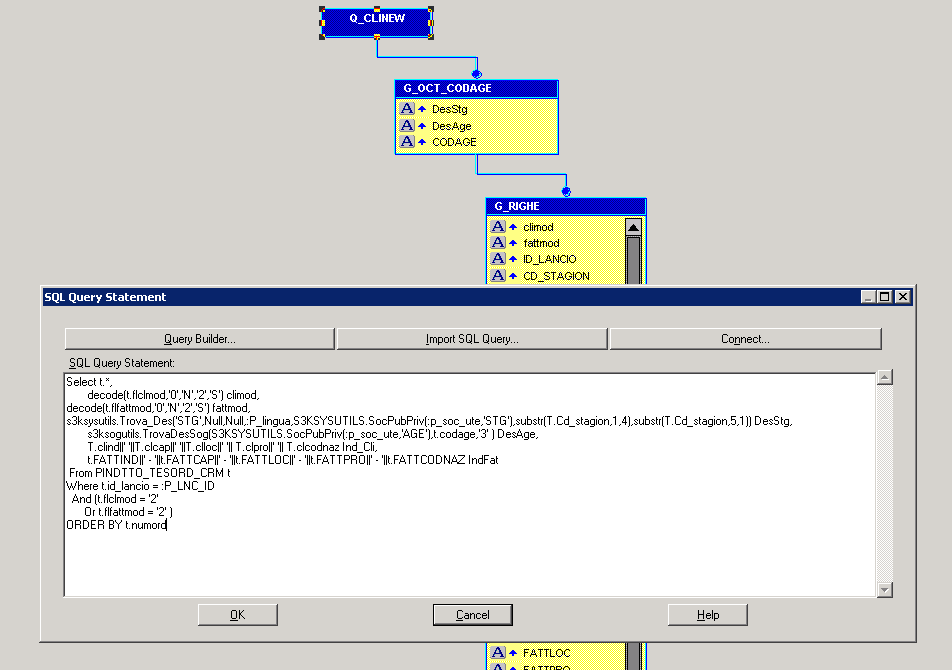
\includegraphics[scale=0.60]{img/QueryRep.png}
\caption{Oracle Reports Builder: Modello da Query}
\end{figure}
\newpage
Sono state inoltre modificate alcune delle program unit ed aggiunte altre, visibili in (figura) per rispondere ad alcune richieste dei Service Manager.\\

\begin{figure}[!h]
\thispagestyle{empty}
\centering
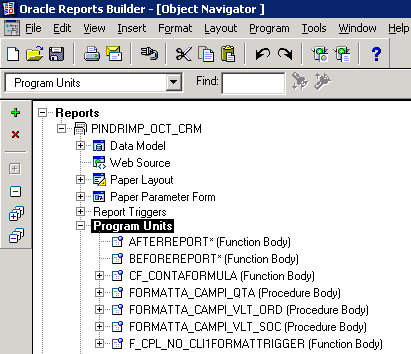
\includegraphics[scale=0.85]{img/RepPU.png}
\caption{Oracle Reports Builder: Program Unit}
\end{figure}
In generale l'attività ha richiesto poco tempo avendo il layout in (figura) valido dalla versione attuale, così come il contenuto di alcune program unit.
\begin{figure}[!h]
\thispagestyle{empty}
\centering
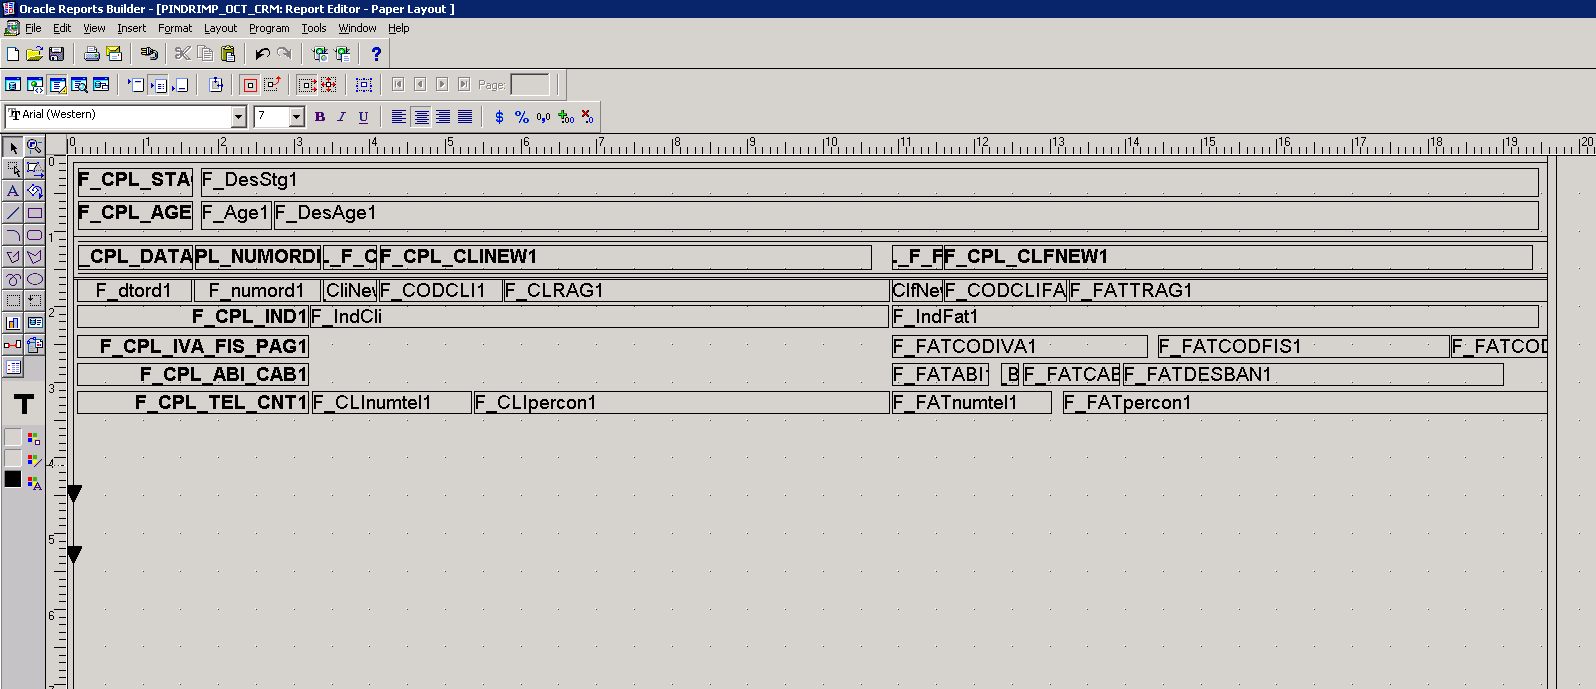
\includegraphics[scale=0.35]{img/ReportDIA.png}
\caption{Oracle Reports Builder: Layout Editor}
\end{figure}